\documentclass[12pt, a4paper]{article}
\usepackage[utf8]{inputenc}
\usepackage{listings}
\usepackage[IL2]{fontenc}
\usepackage[czech]{babel}
\usepackage{graphicx}
\usepackage[export]{adjustbox}
\usepackage[hidelinks]{hyperref}
\usepackage{url}
\usepackage{breakurl}
\usepackage{listings}
\usepackage[final]{pdfpages}
\usepackage{float}
\usepackage{mathtools}


\lstset{
basicstyle=\ttfamily,
frame=single
}

\title{\textbf{Dokumentace semestrální práce} \\KIV/WEB}
\author{Jan Čarnogurský}
\begin{document}

\begin{titlepage}
	\newcommand{\HRule}{\rule{\linewidth}{0.3mm}}
	\begin{center}
	
\includegraphics[width=6cm]{img/logo}\\
	\textsc{\LARGE Západočeská univerzita v Plzni}\\[1.5cm]
	\end{center}
	\textsc{\Large Vyhledávání informací}\\[0.5cm]
	\textsc{\large KIV/IR}\\[0.5cm]
	\HRule\\[0.2cm]
	\begin{center}
	{\bfseries Implementace vlastního systému automatické indexace a vyhledávání dokumentů}\\[0.5cm]
	\end{center}
	\HRule\\[1.5cm]


	\begin{minipage}{\textwidth}
		\begin{flushleft}
			{\Large Čarnogurský Jan\par}
			{\Large A19N0025P\par}
			{\Large cagy@students.zcu.cz\par}
		\end{flushleft}
	\end{minipage}
	\vfill\vfill\vfill
	\begin{flushright}
	{\large\today}
	\end{flushright}
	\vfill
\end{titlepage}

\tableofcontents
\thispagestyle{empty}
\clearpage

\newpage
\section{Zadání}
\subsection{Minimální nutná funkčnost semestrání práce pro získání 15 bodů/zápočtu}
\noindent Tokenizace, Preprocessing (stopwords remover, stemmer/lemmatizer), vytvoření in-memory invertovaného indexu, tf-idf model, cosine similarity,  vyhledávání pomocí dotazu vrací top x výsledků seřazených dle relevance, vyhledávání s pomocí logických operátorů AND, OR, NOT, podrobná dokumentace (programátorská i uživatelská), podpora závorek pro vynucení priority operátorů.

Semestrální práce musí umožňovat zaindexování poskytnutých dat a dat stažených na cvičení (1. cvičení Crawler).

\subsection{Nadstandardní funkčnost (lze získat až dalších 15 bodů)}
Vytvořte účetní aplikaci s následujícími funkcemi:
\begin{itemize}
	\item File-based index (1b)
	\item pozdější doindexování dat (1-2b) - přidání nových dat do existujícího indexu
	\item ošetření např. HTML tagů (1b)
	\item detekce jazyka dotazu a indexovaných dokumentů (1b)
	\item vylepšení vyhledávání (1-?b)
	\item vyhledávání frází (i stop slova)(1b)
	\item vyhledávání v okolí slova (1b)
	\item více scoring modelů (1b)
	\item indexování webového obsahu (2-3b) - zadam web, program stahne data a rovnou je zaindexuje do existujícího indexu
	\item další předzpracování normalizace (1b)
	\item GUI/webové rozhraní (2b)
	\item napovídání keywords (1b)
	\item podpora více polí pro dokument (např. datum, od do)(1b)
	\item CRUD indexovaných dokumentů (2b)
	\item zvýraznění hledaného textu v náhledu výsledků (1b)
	\item dokumentace psaná v TEXu (1b)
	\item implementace dalšího modelu (použití sémantických prostorů) (1-?b)
	\item atd. (xb)
\end{itemize}

\newpage
\section{Analýza}

\subsection{Fulltextové vyhledávání}
\noindent Je speciální způsob vyhledávání informací v databázích nebo v textových souborech, které jsou obvykle předem připraveny, tj. indexovány, aby bylo možno nalézt libovolné slovo (řetězec znaků) v nejkratším možném čase. Při full-textovém vyhledávání vyhledávací algoritmus prozkoumává všechna slova v každém uloženém dokumentu a pokouší se je porovnat se slovy zadanými uživatelem a pokouší se nalézt nejrelevantnější výsledky k zadanému dotazu.

\subsection{Invertovaný index}
\noindent je datová struktura používaná pro fulltextové vyhledávání. Struktura obsahuje mapování obsahu, jako jsou slova nebo čísla. Index se typicky skládá ze slovníku, kde každé slovo obsahuje seznam dokumentů v kterých se vyskytuje. Pro dané slovo lze tedy triviálně zjistit, které dokumenty mu odpovídají.


\subsection{TF-IDF}
\noindent TF-IDF (termín frekvence inverzní frekvence dokumentu) je statistické měřítko, které vyhodnocuje, jak relevantní slovo je pro dokument ve sbírce dokumentů. To se provádí vynásobením dvou metrik: kolikrát se slovo objeví v dokumentu a inverzní frekvence dokumentu slova v sadě dokumentů.

Funguje tak, že se úměrně zvyšuje, kolikrát se slovo objeví v dokumentu, ale je kompenzováno počtem dokumentů, které toto slovo obsahují. Slova, která jsou běžná v každém dokumentu, jako je \uv{tento}, \uv{co}, \uv{a pokud}, mají nízké hodnocení, i když se mohou objevit mnohokrát, protože pro relevanci dokumentu nic neznamenají.

\paragraph{Term frequency (TF)}
\noindent Kolikrát se dané slovo vyskytlo v dokumentu.

\paragraph{Inverse document frequency (IDF)}
\noindent Jak běžné nebo vzácné je slovo v celé sadě dokumentů. Čím blíže je hodnota k 0, tím je slovo běžnější. Tato metrika lze vypočítat tak, že se vezme celkový počet dokumentů, a vydělí se počtem dokumentů, které obsahují slovo.

\paragraph{}
\noindent Vynásobením těchto dvou čísel dostaneme TF IDF ohodnocení slova v daném dokumentu.. Vyšší ohodnocení znamená, že slovo je více relevantní pro dokument.

Ohodnocení TF IDF pro slovo \textit{t} v dokumetu \textit{d}, ze skupiny dokumentů \textit{D} je vypočítáno následovně:

\begin{equation}
tfidf(t,d,D) = log\textsubscript{10}(1 + tf(t,d)) \cdot idf(t,D)
\end{equation}

\subsection{Vector space model}
\noindent Je algebraický model pro reprezentaci textových dokumentů (a všech objektů obecně) jako vektor identifikátorů. Ve vyhledávání je tento model použit pro reprezentaci dokumentů, kde každý dokument je reprezentován váhami TF-IDF, kde řádky jsou definovány slovy v dokumentu. Velikost vektoru tedy odpovídá všem slovům napříč všemi dokumenty. Pokud se dané slovo v dokumentu nevyskytuje, je hodnota TF-IDF pro dané slovo v dokumentu 0.

Jako metrika pro výpočet ohodnocení mezi dvěma vektory se používá \textit{kosínova podobnost}.

\begin{figure}[H]
  \centering
  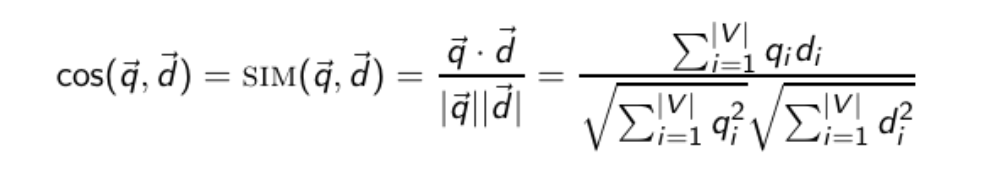
\includegraphics[scale=0.3]{img/cosine.png}
  \label{struktura}
\end{figure}

\begin{description}

	\item [$q_i$] - váha TF-IDF slova \textit{i} v dotazu
	\item [$d_i$] - váha TF-IDF slova \textit{i} v dokumentu
	\item [$\mid \overrightarrow{q} \mid$] a $\mid \overrightarrow{d} \mid$ jsou normalizované délky $\overrightarrow{q}$ a $\overrightarrow{d}$
\end{description}


\subsection{Boolean vyhledávání}
\noindent Booleovský dotaz se skládá z atomů (slova, základní dotazy), které jsou spojeny booleovskými operátory. Odpověď na dotaz je pak sada dokumentů. Dokument buď vyhovuje dotazu, nebo ne, to znamená, že tato metoda neumožňuje rozhodnout, který dokument je pro uživatele relevantnější než druhý.


\noindent Nejčastěji používanými booleovskými operátory jsou:

\paragraph{OR: term1 OR term2}
Dotaz vrací sadu dokumentů, ve kterých je přítomen term1 nebo term 2

\paragraph{AND: term1 AND term2}
Získaná sada se skládá z dokumentů, které obsahují term1 a term2.

\paragraph{NOT: term1 NOT term2}
Dotaz NOT vrací sadu dokumentů, ve kterých je term1 přítomen, ale term2 není.

















\section{Implementace}

\subsection{Invertovaný index}
\noindent Níže jsou popsány třídy, které tvoří strukturu invertovaného indexu.

\subsubsection{Třída InvertIndex}
\noindent Třída představuje samotný invertovaný index. Obsahuje mapu ve spojení \textit{slovo - InvertedIndexItem}. Třída dále obsahuje informaci o tom, jaký typ dat index obsahuje a počet indexovaných dokumentů.


\subsubsection{Třída InvertIndexItem}
\noindent Třída slouží pro držení informací o daném slově. Obsahuje informace o tom, v kterých dokumentech se slovo vyskytuje. Objekt tedy obsahuje mapu ve spojení \textit{dokumentID - WordStats}. Dále se v objektu drží informace o hodnotě \texttt{IDF} slova.

\subsubsection{Třída WordStats}
\noindent Obashuje statistiky pro slovo v dokumentu. Třída tedy obsahuje informaci o tom, kolikrát se dané slovo v dokumentu vyskytlo, hodnotu \texttt{TF-IDF} a referenci na \textit{DocumentBag}.

\subsubsection{Třída DocumentBag}
\noindent Představuje obal nad zaindexovaným dokumentem. Třída obsahuje seznam všech slov v dokumentu a vypočítanou euklidovskou střední hodnotu. Tím, že třída obashuje seznam všech slov v dokumentu, značně urychlý proces indexování, protože při výpočtu euklidovské střední hodnoty, není nutné procházet celý slovník a kontrolovat, zda dané slovo obsahuje dokument.

\subsubsection{Načtení dat}
\noindent Pro načtení dat jsou implementovány třídy, které implementují rozhraní \texttt{ILoader}. Pro získání správné třídy pro načtení dat je implementována továrna \texttt{LoaderFactory}, která na základě předaného výčtového typu \texttt{ELoader\-Type} vrátí příslušnou třídu. Cesty k jednotlivým souborům, které jsou třídami načítány jsou nastavené ve třídě \texttt{Config} a jsou předány konstruktorem v továrně.

\subsubsection{Preprocessing}
\noindent Pro preprocessing byla zvolena následující konfigurace:
\begin{itemize}
	\item ignorování stop slov
	\item pro stematizaci byl zvolen \texttt{CzechStemmerLight}
	\item pro tokenizaci byl zvolen \texttt{AdvancedTokenizer}
	\item odstranění akcentu po stematizaci
	\item převod na lowercase
	\item ignorování slov menších než 2
\end{itemize}


\subsubsection{Uložené informace}
\noindent Do indexu jsou spočítány následující informace, které se sním ukládají:
\begin{itemize}
	\item základní struktura (slovo-dokument)
	\item euklidovská střední hodnota dokumentů, to znamená, že i její všechny mezivýpočty (\texttt{IDF}, \texttt{TF-IDF}, ...)
\end{itemize}

\subsubsection{Princip vytvoření indexu}
\noindent Na základě požadovaných dat se vybere třída pro načítání dat. Data se načtou, a předají se do indexu pro indexování. V průběhu indexace se procházejí načtená data, kde se průběžně obsah dokumentů vkládá do preprocessingu, který vrátí list upravených slov dokumentu pro indexaci. Tyto slova jsou postupně vkládána do invertovaného seznamu a také do \texttt{DocumentBagu} pro daný dokument (vždy se indexují slova jen pro jeden dokument, takže během zpracování jednoho dokumentu se vytvoří právě jeden \texttt{DocumentBag}). Po uložení všech slov dokumentů do invertovaného indexu se uloži jeho \texttt{DocumentBag} do listu pro pozdější vypočítání euklidovské střední hodnoty. Po zaindexování všech dokumentů do invertovaného indexu, jsou nastaveny ke slovům váhy \texttt{IDF} a \texttt{TD-IDF}, následně jsou vypočítány euklidovské střední hodnoty dokumentů (zde se prochází list uložených \texttt{DocumentBagů}, aby nebylo nutné hledat všechny unikátní dokumenty). Indexu se ještě nastaví informace o tom, jaké data jsou zaindexována. Po dokončení indexace je index uložen do souboru.

\subsubsection{Načítání uloženého indexu}
\noindent Jelikož je implementováno GUI, provádí se indexace ve dvou třídách. První je třída \texttt{TestTrecEval}, která slouží především pro kontrolu výsledků. Zde je iplementována podmínka, kde je nutné ručně změnit, jestli je poždadováno zaindexovat data, nebo ručně načíst data ze souboru. Pokud jsou data indexována, celý průběh i s uložením trvá okolo 100 sekund. Defaultně se data vždy indexují.

Implementace načítání dat v GUI je popsána v kapitole \ref{gui-index}

\subsection{Vyhledávání}

\subsubsection{Výběr vyhledávače}
\noindent Pro vyhledávání jsou implementovány třídy, které implementují rozhraní \texttt{Searcher}. Pro získání správné třídy pro vyhledávání je implementována továrna \texttt{SearcherFactory}, která na základě předaného výčtového typu \\\texttt{ESearchType} vrátí příslušnou třídu.

\subsubsection{VSM}
\noindent Pro tento způsob vyhledávání je implementována třída \texttt{VectorSpaceModel\-Searcher}. Třída nejdříve zaindexuje dotaz (\textit{indexQuery()}) do vlastního slovníku a spočte \texttt{TF-IDF} hodnoty pro slova v dotazu a celkovou euklidovskou střední hodnotu.

Následně jsou získány všechny \texttt{DocumentBagy} všech dokumentů, ve kterých se vyskytuje některé slovo z dotazu. Potom je zavolána metoda \textit{getResults()}, která spočte kosínovu podobnost pro \texttt{DocumentBag} dotazu s \\\texttt{DocumentBagy} dokumentů a seřadí je od nejrelevantnějších.

\subsubsection{Boolean}
\noindent Pro tento způsob vyhledávání je implementována třída \texttt{BooleanSearcher}. Pro parsování boolean dotazu byla použita knihovna \textit{Lucene}, přesněji její třída \texttt{PrecedenceQueryParser}, která se postará o prioritu operátorů. Následně se v cyklu prochází listy jednotlivé subdotazy, které volají metodu \textit{processQuery()}, která se postará o další operace (OR, AND, NOT). Pokud subdotaz obsahuje nějaký další subdotaz, metoda se volá rekurzivně, dokud nedojde k hodnotě (slovu).

\subsection{GUI}
\noindent Pro implementaci GUI byla zvolena knihovna \textit{JavaFX}. GUI obsahuje dvě okna, jedno pro vyhledávání (\texttt{AppController}) a druhé pro editaci záznamů (\texttt{EditController}).

\subsubsection{Spuštění}\label{gui-index}
\noindent Aplikace zkontroluje jestli existuje uložený invertovaný index. Pokud ano, pokusí se soubor načíst. Pokud je soubor úspěšně načten, označí typ načtených dat a je možné vyhledávat. Pokud čtení souboru skončí chybou nebo soubor neexistuje, aplikace zaindexuje znovu data. Defaultní hodnota dat, které se indexují je možné změnit v třídě \texttt{Config}.

\subsubsection{Vyhledávání dat}
\noindent Při vyhledávání se načtou zvolené hodnoty radiobuttonů (typ vyhledávání, typ dat ve kterých vyhledávat). Nejdříve se zkontroluje, jestli zvolený typ dat je načten v paměti, pokud není, provede se indexování požadovaných dat.

Pokud je index v pořádku, nebo po zaindexování nových dat, se získá příslušný vyhledávač, podle typu vyhledávání a provede se vyhledávání. V seznamu pod vyhledáváním se zobrazí 10 nejrelevantnějších výsledků.

\subsubsection{CRUD dat a doindexování}\label{crud}
\noindent CRUD dat je možný ve správě dat. Po provedení změn je nutné data uložit a zaindexovat, pokud se změny neuloží nebudou promítnuty a budou ignorovány. Omezení, které tato implementace má je ta, že data které se načítají pro zobrazení informací (nastavení nového titulku) se drží jenom v paměti. Takže pokud se aplikace ukončí a znovu načte, index se načte se změnou, to znamená, že pokud budu hledat dokument podle nového titulku tak ho naleznu, ale v detailu se mi zobrazí starý titulek.

Je ošetřeno pokud uživatel bude chtít přidat další dokument s duplicitním ID, nebo editovat ID na existující ID. Kontrola, jaký dokument se má upravit/smazat je řešena přes krytý label, do kterého se ukládá původní hodnota ID. Výsledky operací jsou zobrazeny ve spodní části okna.

\section{Uživatelská příručka}
\subsubsection{Start aplikace}
\noindent Pro start aplikace není nutné zadávat žádný parametr, pokud bude existovat uložený invertovaný index, aplikace se ho pokusí sama načíst. Po načtení by se mělo zobrazit následující okno aplikace. Hodnota typu dat se přepne podle aktuálně načteného indexu.

\begin{figure}[H]
  \centering
  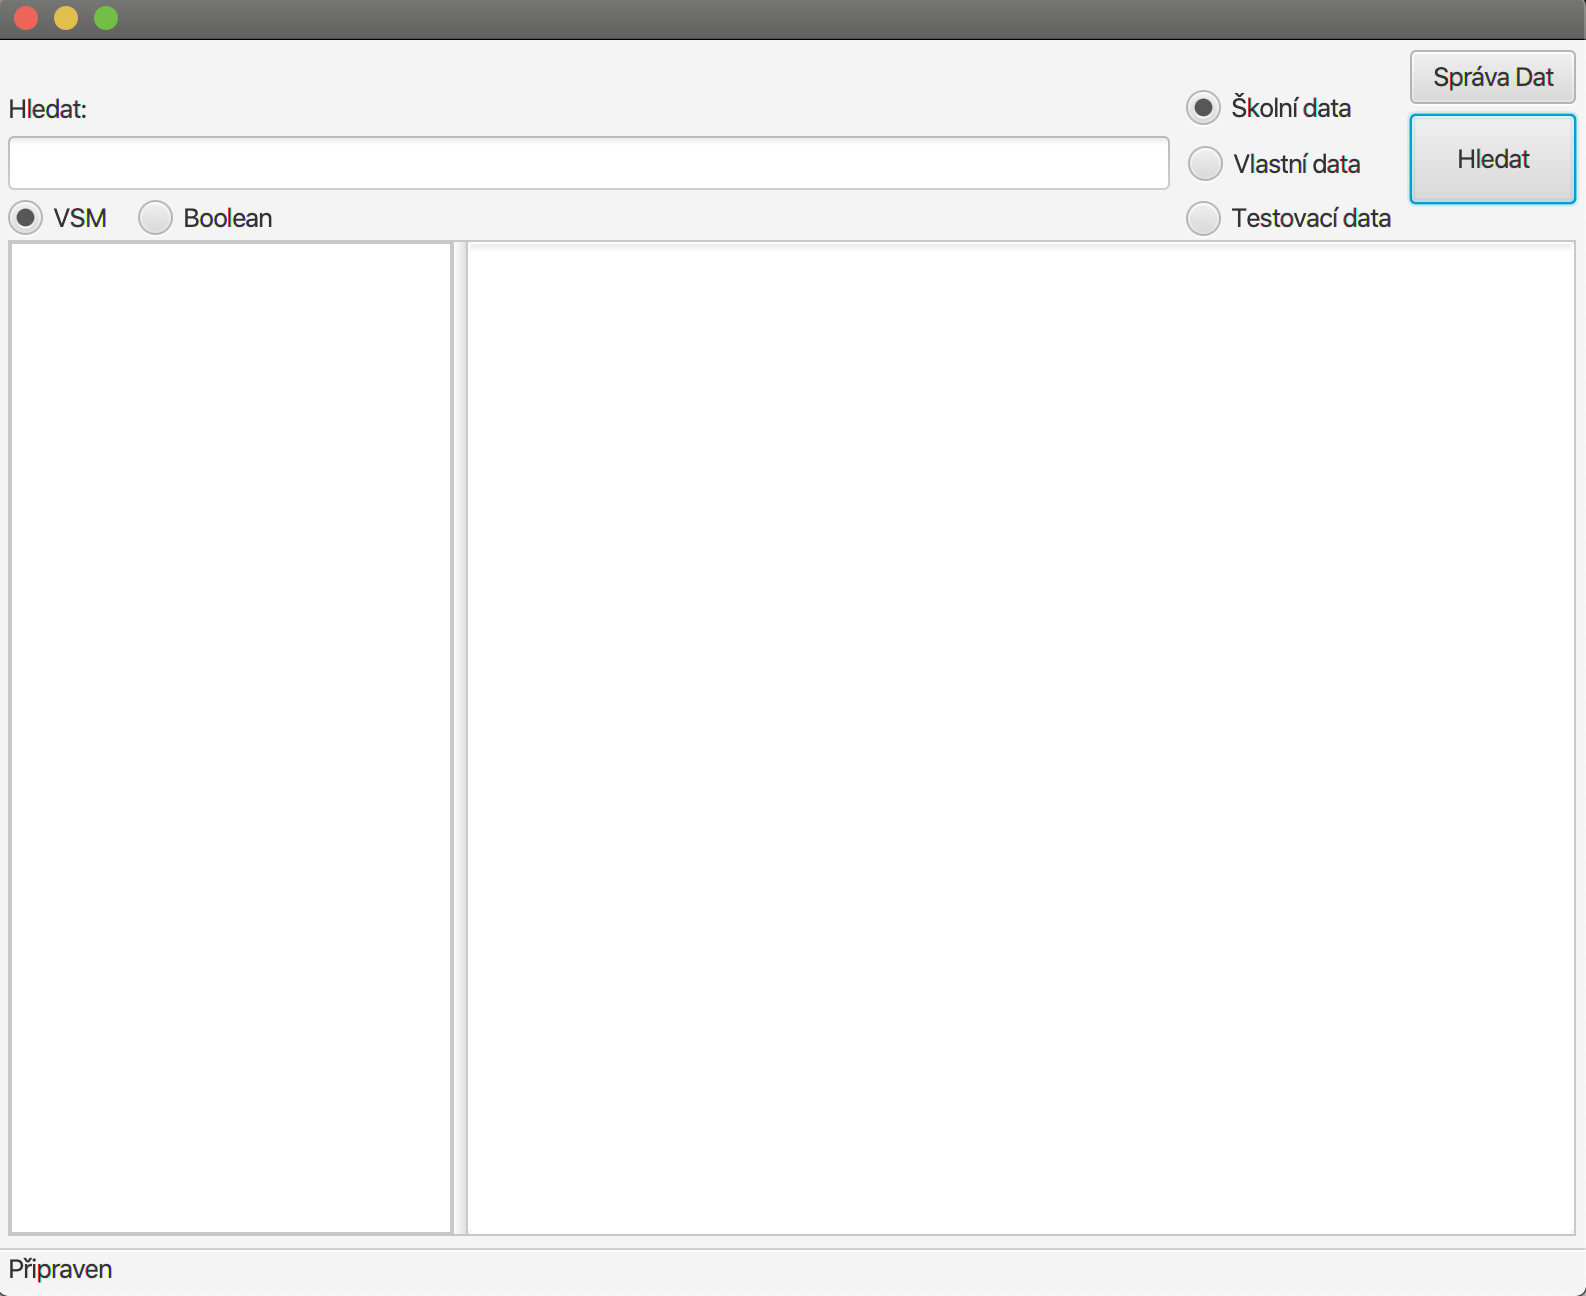
\includegraphics[scale=0.5]{img/start.png}
  \caption{Apliakce po spuštění}
\end{figure}
\newpage
\subsection{Vyhledávání}
\noindent Vyhledávání je možné zadáním dotazu do vstupního pole. Je možné si vybrat, jestli se má vyhledávat pomocí VSM nebo Boolean dotazu. Dále je možné vybrat typ dat. Pokud dojde ke změně typu dat, aplikace si na pozadí zaindexuje požadovaná data, proto se může stát, že aplikace na chvíli zamrzne. Zobrazuje se 10 nejrelevantnějších výsledků. Celkový počet výsledků je zobrazen ve spodní části okna. Kliknutím na výsledek se zobrazí jeho detail.

\begin{figure}[H]
  \centering
  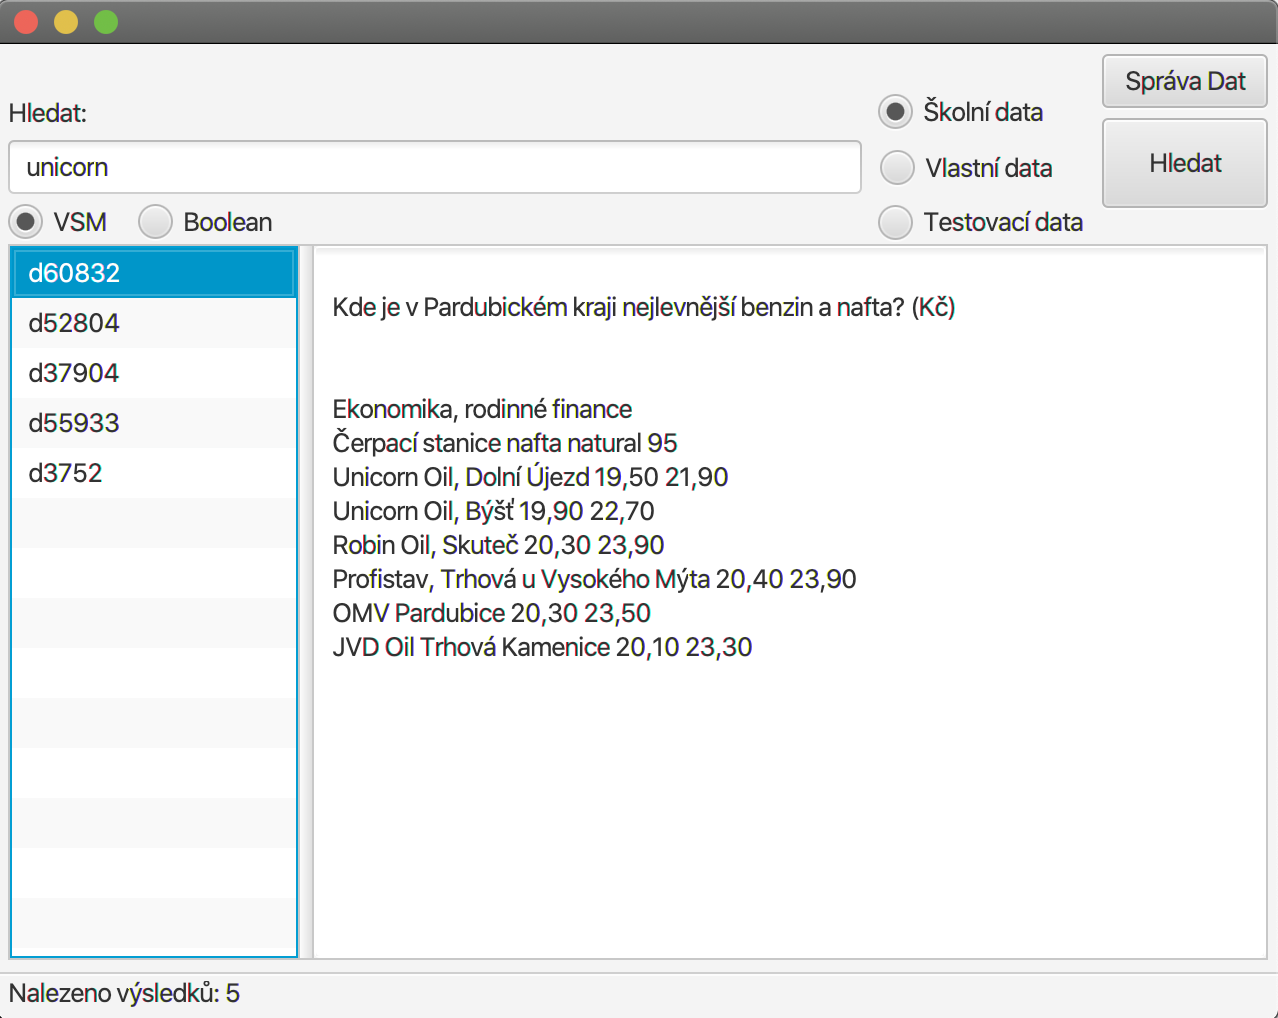
\includegraphics[scale=0.5]{img/search.png}
  \caption{Ukázka vyhledávání}
\end{figure}

\newpage
\subsubsection{Editace}
\noindent Editace dokumentů je možná stisknutím tlačítka \uv{Správa dat} vpravé horní části okna. Je možné provádět všechny CRUD operace. Po provedení změn je nutné změny uložit a zaindexovat, jinak budou ignorovány. Po uložení změn je možné se vrátit zpět do hlavního okna tlačítkem \uv{Zpět}.

Pro vložení nového záznamu je nutné vyplnit alespoň unikátní ID dokumentu. Pro upravení/smazání je nutné nejprve vybrat dokument.

\begin{figure}[H]
  \centering
  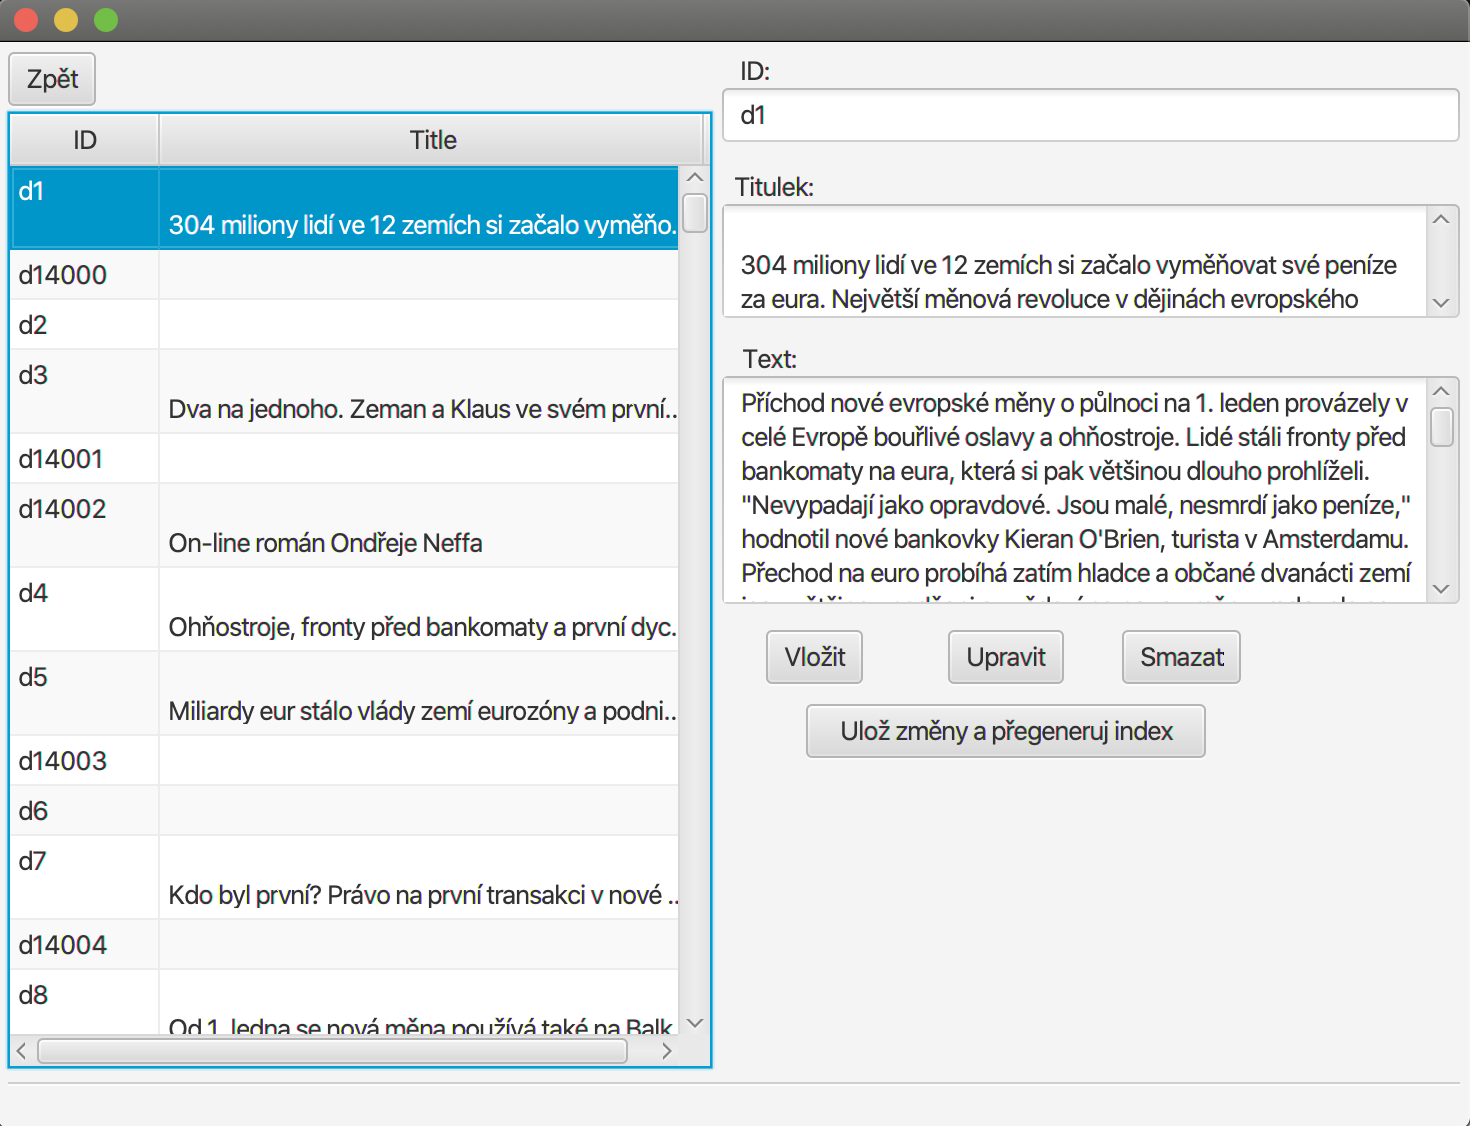
\includegraphics[scale=0.5]{img/edit.png}
  \caption{Editace}
\end{figure}
\newpage
\section{Závěr}
\noindent Aplikace splňuje minimální požadavky semestrální práce. Nad rámec zadání byly implementovány funkčnosti:

\begin{itemize}
	\item File-based index
	\item Pozdější doindexování dat
	\item GUI/webové rozhraní
	\item CRUD indexovaných dokumentů
	\item Dokumentace psaná v TEXu
\end{itemize}

\noindent Podle výsledků hodnota map odpovídá hodnotě 0,1701. Měření bylo omezeno pro 1000 výsledků na dotaz a hledalo se podle nadpisu a popisu.

\begin{figure}[H]
  \centering
  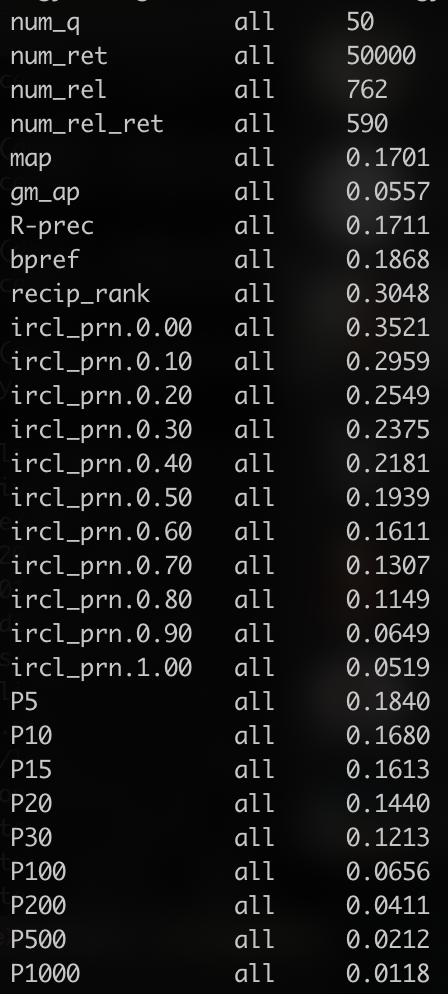
\includegraphics[scale=0.5]{img/result.png}
  \label{struktura}
\end{figure}

Největší problém s kterým jsem se při implementaci setkal bylo \uv{správné} vyhodnocení boolean dotazu. Implementaci jsem převážně testoval na testovacích datech. Ukázky dotazů které jsem úspěšně otestoval jsou ukázány v třídě \texttt{BooleanSearcher}.

Snažil jsem se projekt strukturovat tak, aby byl přehledný, a proto jsem trochu pozměnil zadané rozhraní. Jelikož se ale jednalo jen o možnou šablonu, tak doufám, že to nebude problém.

Projekt je vedený na \href{https://github.com/cagysek/IncredibleElastic}{GITu}.


\end{document}
